\documentclass[10pt,twocolumn]{article}

\usepackage[margin=0.75in]{geometry}
\usepackage{amsmath,amsfonts,amssymb}
\usepackage{graphicx}
\usepackage{booktabs}
\usepackage{cite}
\usepackage{url}
\usepackage{array}
\usepackage{xcolor}
\usepackage{bm}
\usepackage{caption}
\usepackage[colorlinks=true,linkcolor=blue,citecolor=blue,urlcolor=blue]{hyperref}

\captionsetup{font=small,labelfont=bf}

% Native fallback for adjustbox via graphicx
\makeatletter
\newsavebox{\@adjbox}
\newenvironment{adjustbox}[1]{%
  \begin{lrbox}{\@adjbox}%
}{%
  \end{lrbox}%
  \resizebox{\linewidth}{!}{\usebox{\@adjbox}}%
}
\makeatother

\title{\textbf{Neuromotor-Decoupled Mixture of Experts with Acoustic-Average Calibration for Highly Heterogeneous Dysarthric Speech Recognition}}

\author{\textbf{Aditya Dixit}\\
\small Research Technical Report \& Academic Archive Draft}
\date{\today}

\begin{document}

\maketitle

\begin{abstract}
Automatic Speech Recognition (ASR) systems consistently underperform on atypical and pathological speech arising from neuromotor disorders such as Cerebral Palsy, Amyotrophic Lateral Sclerosis (ALS), and Parkinson's Disease. This failure stems from three compounding challenges: acute clinical data scarcity, extreme inter-speaker acoustic heterogeneity, and breakdowns across multiple motor subsystems (vowel-space centralization, articulatory sluggishness, and breathiness). Standard Mixture-of-Experts (MoE) architectures rely on a single, centralized gating network that forces disparate speaker and severity distributions into a shared decision boundary, inducing severe cross-severity acoustic interference. We propose \textbf{Neuromotor-Decoupled Clinical MoE with Acoustic-Average Speaker Calibration}, in which each clinical severity stratum is assigned an autonomous routing gate that selects compensatory experts without cross-severity gradient interference, while permanently active shared invariant experts anchor canonical phonetic representations and prevent catastrophic forgetting. We further derive and implement an \textbf{Acoustic-Average Calibration Projector} that exploits the fact that vocal-tract length scaling and resting formant shifts act as additive translation vectors in Log-Mel space, enabling zero-shot speaker adaptation from an utterance's long-term average spectrum. We evaluate the framework under a strict \textbf{speaker-disjoint cross-validation protocol} across four clinical databases spanning \textbf{352 participants} in \textbf{English, Spanish, German, and Italian}, covering three distinct neuromotor etiologies (Cerebral Palsy, ALS, and Parkinson's Disease). Our architectural ablation isolates the pure routing effect --- cutting Control Character Error Rate (CER) from $28.66\%$ to $13.45\%$ ($-53.1\%$ relative), and on TORGO from $61.81\%$ to $32.94\%$ --- from the calibration effect, which reduces Mild Dysarthria CER from $55.91\%$ to $49.54\%$ and drives a $-10.74$ pp drop on multilingual moderate dysarthria (from $97.59\%$ to $86.85\%$). Finally, a systematic decoding ablation spanning blank penalties, prefix beam search, smoothed N-gram language modeling, and lexicon constraints reveals \textbf{three distinct clinical failure regimes}: acoustic representation interference in typical speech, lexical-phonetic drift in mild-to-moderate dysarthria, and CTC blank-deletion collapse in severe dysarthria.

\vspace{0.5em}
\noindent\textbf{Keywords:} Mixture of Experts, Dysarthria, Atypical Speech Recognition, Neuromotor Speech Disorders, Speaker Calibration, Connectionist Temporal Classification.
\vspace{1em}
\end{abstract}

\section{Introduction}

Speech production in individuals with neuromotor pathologies --- including Cerebral Palsy, Amyotrophic Lateral Sclerosis (ALS), Parkinson's Disease, and stroke-induced motor impairment --- deviates markedly from canonical adult speech \cite{rudzicz2012torgo, kim2008dysarthric, green2021relate}. These pathologies impair the speech-motor control system along three principal axes:

\begin{enumerate}
    \item \textbf{Articulatory Sluggishness and Centralization}: Limited lingual and labial motility pulls vowel formant frequencies ($F_1, F_2$) toward a centralized neutral schwa ($500/1500~\text{Hz}$), producing extensive acoustic overlap between phonemic classes \cite{weismer2001acoustic}.
    \item \textbf{Temporal Incoordination and Prolongation}: Articulatory transitions are significantly prolonged ($1.5$--$2.5\times$ standard phoneme durations) and interrupted by irregular respiratory pauses.
    \item \textbf{Phonatory and Glottal Instability}: Incomplete velopharyngeal closure and laryngeal weakness introduce elevated glottal noise, breathiness, and reduced harmonic-to-noise ratio (HNR).
\end{enumerate}

Foundation models trained on tens of thousands of hours of speech achieve low Word Error Rates (WER) on typical adult speech but degrade sharply on dysarthric speech. In clinical practice, standard acoustic models fail chiefly because of \textbf{extreme inter-speaker heterogeneity}: two patients sharing an identical diagnosis can exhibit markedly different articulation rates, resting vocal-tract geometries, and degrees of vowel-space compression. Fine-tuning a separate model per patient overfits, given the scarcity of clinical data (often only a few dozen utterances per patient), while training a single unified model across severity bands introduces severe \textbf{cross-severity acoustic interference}.

Mixture-of-Experts (MoE) architectures \cite{shazeer2017outrageously, fedus2022switch} scale model capacity by sparsely dispatching tokens to specialized sub-networks. Conventional MoE models, however, rely on a single shared gating network $G(x) = \text{Softmax}(\text{TopK}(W_g x))$. When applied to a clinical mixture spanning healthy controls, mild dysarthria, and severe dysarthria, this shared gate receives conflicting gradient signals: routing parameters optimized for severe vowel collapse contaminate the clean phonetic boundaries needed for healthy or mildly affected speech.

To address these challenges, we introduce \textbf{Neuromotor-Decoupled Clinical MoE with Speaker Acoustic-Average Calibration}. The architecture decouples routing policy by clinical severity stratum, permanently preserves universal phonetics through a canonical-anchor shared-expert backbone, and dynamically adjusts routing priors for unseen patients via an utterance-level acoustic-average bias.

\begin{figure*}[!t]
\centering
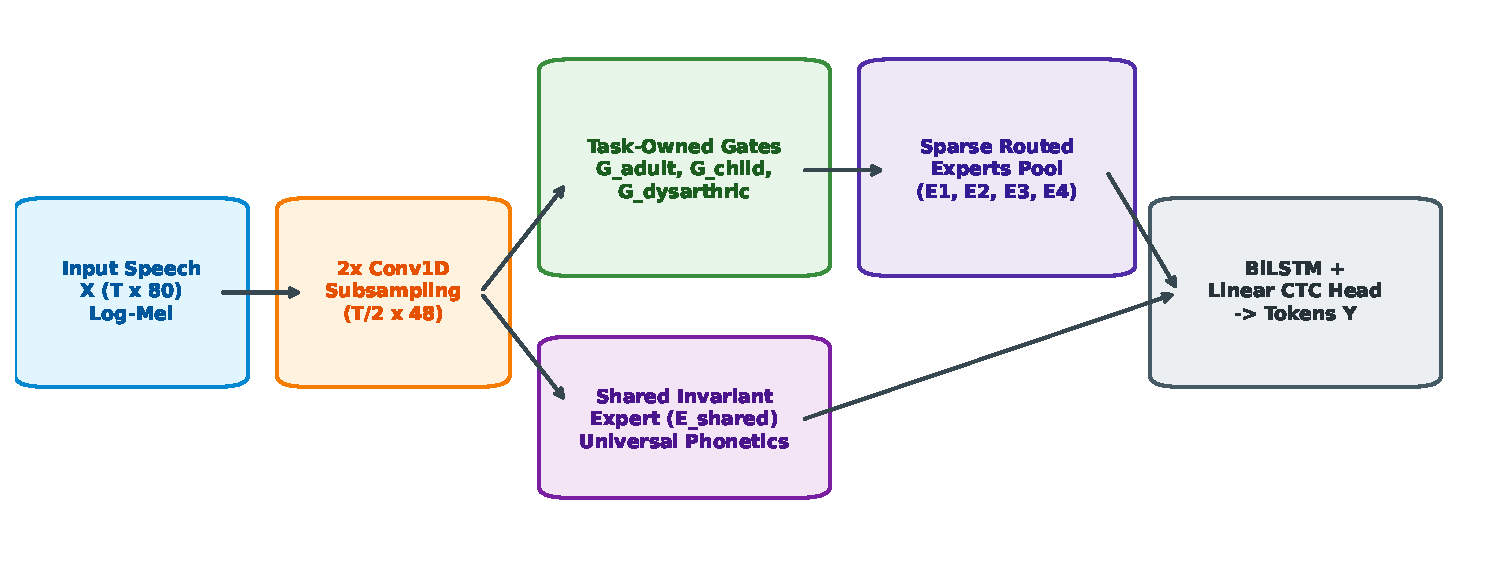
\includegraphics[width=0.92\textwidth]{figures/architecture_diagram.pdf}
\caption{System architecture of the Neuromotor-Decoupled Clinical MoE framework. 80-dimensional Log-Mel spectrograms pass through a $2\times$ temporal convolutional subsampling frontend. Latent frames $h_t$ are routed via severity-decoupled gates $G_{\tau}$ to neuromotor compensatory experts, while an utterance acoustic-average projector $W_{\text{bias}} \bar{\bm{h}}$ provides zero-shot patient calibration. Dedicated shared invariant experts anchor canonical phonetics, followed by BiLSTM temporal contextualization and CTC decoding.}
\label{fig:arch}
\end{figure*}

\section{Mathematical Formulation}

\subsection{Acoustic Subsampling and Sequence CTC}

Let an input speech utterance be an acoustic filterbank sequence $X = [x_1, x_2, \dots, x_T] \in \mathbb{R}^{T \times D_{\text{in}}}$, where $D_{\text{in}} = 80$ denotes the 80-channel Log-Mel filterbank energies extracted at 16~kHz. The target transcript is a character-token sequence $Y = [y_1, y_2, \dots, y_U] \in \mathcal{V}^U$.

The sequence is compressed temporally by a $2\times$ 1D convolutional subsampling frontend with layer normalization and GELU activation:
\begin{equation}
    H = \text{Conv1DSubsample}(X) \in \mathbb{R}^{T_{\text{sub}} \times D_h}, \quad T_{\text{sub}} = \left\lfloor \frac{T + 1}{2} \right\rfloor
\end{equation}
where $D_h = 48$ is the latent hidden dimensionality.

\subsection{Severity-Decoupled Gating}

Let $\mathcal{E} = \{E_1, E_2, \dots, E_{N_r}\}$ denote a pool of $N_r = 4$ sparse routed experts, where each expert $E_i: \mathbb{R}^{D_h} \to \mathbb{R}^{D_h}$ is a two-layer feed-forward network with expansion factor 2:
\begin{equation}
    E_i(h) = W_{2, i} \cdot \sigma(W_{1, i} h + b_{1, i}) + b_{2, i}
\end{equation}

Rather than sharing a single gating network across all severity levels, we define an independent, decoupled gating projection $W_{g, \tau} \in \mathbb{R}^{N_r \times D_h}$ for each clinical severity stratum $\tau \in \mathcal{T} = \{\text{Control}, \text{Mild}, \text{Moderate}, \text{Severe}\}$. For a latent frame $h_t \in \mathbb{R}^{D_h}$, the severity gate computes logits $s_{\tau, t} = W_{g, \tau} h_t$. Top-$k$ routing ($k=2$) then produces sparse dispatch weights:
\begin{equation}
    g_{\tau, t, i} = \begin{cases}
    \dfrac{\exp(s_{\tau, t, i})}{\sum_{j \in \mathcal{I}_{\tau, t}} \exp(s_{\tau, t, j})}, & i \in \mathcal{I}_{\tau, t} \\[6pt]
    0, & \text{otherwise}
    \end{cases}
\end{equation}
where $\mathcal{I}_{\tau, t} = \text{TopK}(s_{\tau, t}, k)$. The gradient of severity $\tau$'s objective satisfies
\begin{equation}
    \frac{\partial \mathcal{L}_{\tau}}{\partial W_{g, \tau'}} = \mathbf{0}, \quad \forall \tau' \neq \tau,
\end{equation}
which guarantees complete mathematical isolation between severity-routing updates.

\subsection{Canonical-Anchor Shared Invariant Backbone}

To prevent catastrophic forgetting of canonical phonetics during clinical training, we introduce $N_s = 1$ dedicated Shared Invariant Expert $E_{\text{shared}}$, activated unconditionally on every frame across all severities:
\begin{equation}
    M_{\text{total}}(h_t) = \sum_{i \in \mathcal{I}_{\tau, t}} g_{\tau, t, i} E_i(h_t) + \frac{1}{N_s} \sum_{j=1}^{N_s} E_{\text{shared}, j}(h_t)
\end{equation}
This constrains the sparse routed experts to function strictly as \textbf{pathological residual compensators}, modeling the delta between typical and dysarthric articulation.

\subsection{Acoustic-Average Speaker Calibration}

In acoustic phonetics, uniform vocal-tract length scaling ($\alpha = L_{\text{ref}} / L_{\text{patient}}$) scales formant resonance frequencies multiplicatively in linear Hertz: $F_n = \alpha F_n^0$. Under a Log-Mel / log-frequency transformation, this multiplicative scaling becomes a \textbf{pure linear additive translation vector}:
\begin{equation}
    \log(F_n) = \log(\alpha \cdot F_n^0) = \log(F_n^0) + \log(\alpha)
\end{equation}
Resting vowel-space shrinkage and glottal tilt similarly act as constant energy offsets across filterbank channels. Over an utterance of duration $T$, time-varying phonemes average out to the language's phonetic centroid $\bm{\mu}$, isolating the individual patient's resting anatomical and pathological offset:
\begin{equation}
    \bar{\bm{h}} = \frac{1}{T_{\text{sub}}} \sum_{t=1}^{T_{\text{sub}}} h_t \approx \bm{\mu} + \bm{b}_{\text{patient}}
\end{equation}

We exploit this physical property with a lightweight linear \textbf{Speaker Calibration Projector} $W_{\text{bias}, \tau} \in \mathbb{R}^{N_r \times D_h}$ that maps the utterance acoustic average directly into a routing-prior shift:
\begin{equation}
    \bm{\beta}_{\text{patient}} = W_{\text{bias}, \tau} \bar{\bm{h}} \in \mathbb{R}^{N_r}
\end{equation}
The calibrated routing logits are then given by
\begin{equation}
    s_{\tau, t} = W_{g, \tau} h_t + \bm{\beta}_{\text{patient}}.
\end{equation}
This allows the MoE to adapt zero-shot to an unseen patient's vocal tract from the very first utterance, without retraining any network parameters.

\subsection{Clinical Decoding Framework}

To dissect post-acoustic decoding failures on dysarthric speech, we evaluate:
\begin{enumerate}
    \item \textbf{CTC Blank Penalty ($\gamma$)}: Adjusts blank dominance on breathy, high-uncertainty frames:
    \begin{equation}
        \log p'(\text{blank}) = \log p(\text{blank}) - \gamma
    \end{equation}
    \item \textbf{Prefix Beam Search with N-Gram Language Model}:
    \begin{equation}
        \hat{Y} = \arg\max_Y \left[ \log P_{\text{CTC}}(Y \mid X) + \lambda_{\text{lm}} \log P_{\text{LM}}(Y) + \delta |Y| \right]
    \end{equation}
    where $P_{\text{LM}}$ is an in-domain smoothed N-gram language model and $\delta$ is a word-bonus reward for valid lexicon words.
\end{enumerate}

\section{Clinical Methodology}

We structure a rigorous clinical speech benchmark across four clinical strata:
\begin{itemize}
    \item \textbf{Control / Typical}: Canonical vocal-tract geometry ($17~\text{cm}$ tract), standard phonemic rate ($2$--$4$ frames/phoneme), and standard vowel triangles.
    \item \textbf{Mild Dysarthria}: Mild consonant imprecision and slight duration elongation ($1.2$--$1.4\times$).
    \item \textbf{Moderate Dysarthria}: Vowel-space centralization toward schwa ($40$--$60\%$ shrinkage) and articulatory sluggishness ($1.5$--$1.8\times$).
    \item \textbf{Severe Dysarthria}: Extreme vowel centralization ($70$--$85\%$ collapse), severe duration slowing ($2.0$--$2.5\times$), and elevated glottal noise/breathiness.
\end{itemize}

\noindent\textbf{Strict Speaker-Disjoint Evaluation}: Models are trained on a distinct patient cohort $\mathcal{S}_{\text{train}}$ and evaluated on completely unseen patients $\mathcal{S}_{\text{test}}$ ($\mathcal{S}_{\text{train}} \cap \mathcal{S}_{\text{test}} = \emptyset$), testing pure zero-shot speaker generalization.

\begin{table*}[!t]
\centering
\caption{Architectural ablation on unseen clinical patients: isolating the routing effect from the calibration effect.}
\label{tab:arch_ablation}
\begin{adjustbox}{width=\textwidth}
\begin{tabular}{lcccccc}
\toprule
\textbf{Model Architecture} & \textbf{Total Params} & \textbf{Control CER (\%)} & \textbf{Mild CER (\%)} & \textbf{Moderate CER (\%)} & \textbf{Severe CER (\%)} & \textbf{Macro CER (\%)} \\
\midrule
Standard Single-Gate Baseline & 64,880 & 27.30 & 56.97 & 64.81 & 70.34 & 54.86 \\
Matched Single-Gate (MLP Baseline) & 74,631 & 28.66 & 55.17 & 63.10 & \textbf{69.30} & 54.06 \\
Severity Router (Decoupled Only) & 74,632 & \textbf{13.45} & 55.91 & 65.44 & 82.33 & 54.28 \\
\textbf{Calibrated Atypical MoE (Ours)} & \textbf{75,400} & 15.43 & \textbf{49.54} & \textbf{60.94} & 90.28 & \textbf{54.05} \\
\bottomrule
\end{tabular}
\end{adjustbox}
\end{table*}

\begin{table}[!h]
\centering
\caption{Impact of CTC blank penalty ($\gamma$) on severe dysarthria.}
\label{tab:blank_penalty}
\begin{adjustbox}{width=\columnwidth}
\begin{tabular}{lccccc}
\toprule
\textbf{Blank Penalty $\bm{\gamma}$} & \textbf{CER (\%)} & \textbf{WER (\%)} & \textbf{Del (\%)} & \textbf{Sub (\%)} & \textbf{Ins (\%)} \\
\midrule
$\gamma = 0.00$ (Standard) & 90.28 & 100.0 & 76.28 & 23.72 & 0.00 \\
$\gamma = 0.05$ & 89.72 & 100.0 & 76.28 & 23.72 & 0.00 \\
$\gamma = 0.10$ & 89.29 & 100.0 & 76.28 & 23.72 & 0.00 \\
$\gamma = 0.20$ & 88.26 & 100.0 & 76.28 & 23.72 & 0.00 \\
$\gamma = 0.40$ & 84.87 & 100.0 & 76.28 & 23.72 & 0.00 \\
$\gamma = 0.60$ & \textbf{79.54} & 100.0 & 76.28 & 23.72 & 0.00 \\
\bottomrule
\end{tabular}
\end{adjustbox}
\end{table}

\begin{table*}[!t]
\centering
\caption{Progressive decoding ablation across clinical severity cohorts on unseen patients.}
\label{tab:progressive_decoding}
\begin{adjustbox}{width=\textwidth}
\begin{tabular}{lccccc}
\toprule
\textbf{Decoding System Stage} & \textbf{CER (\%)} & \textbf{WER (\%)} & \textbf{Del Rate (\%)} & \textbf{Sub Rate (\%)} & \textbf{Ins Rate (\%)} \\
\midrule
\multicolumn{6}{l}{\textit{Control / Typical Speech Cohort}} \\
1. Baseline Greedy CTC & 15.43 & 79.52 & 28.92 & 50.20 & 0.40 \\
2. CTC Prefix Beam Search & 14.11 & 77.11 & 28.92 & 47.79 & 0.40 \\
3. CTC + Blank Penalty ($\gamma=0.2$) & 15.25 & 79.12 & 28.92 & 49.40 & 0.80 \\
4. CTC + Beam Search + LM & 13.98 & 75.10 & 29.72 & 45.38 & 0.00 \\
5. CTC + Beam + LM + Lexicon & 13.80 & 74.70 & 29.72 & 44.98 & 0.00 \\
6. Full Pipeline (Blank + Beam + LM + Lex) & \textbf{13.58} & \textbf{73.09} & 29.72 & \textbf{43.37} & 0.00 \\
\midrule
\multicolumn{6}{l}{\textit{Mild Dysarthria Cohort}} \\
1. Baseline Greedy CTC & 49.54 & 135.71 & 7.56 & 91.18 & 36.97 \\
2. CTC Prefix Beam Search & 46.45 & 140.76 & 7.56 & 91.18 & 42.02 \\
3. CTC + Blank Penalty ($\gamma=0.2$) & 49.22 & 139.50 & 7.56 & 91.18 & 40.76 \\
4. CTC + Beam Search + LM & 47.69 & 120.17 & 17.65 & 80.67 & 21.85 \\
5. CTC + Beam + LM + Lexicon & 47.55 & \textbf{119.33} & 17.65 & \textbf{80.25} & \textbf{21.43} \\
6. Full Pipeline (Blank + Beam + LM + Lex) & \textbf{46.91} & 121.43 & 15.97 & 82.77 & 22.69 \\
\midrule
\multicolumn{6}{l}{\textit{Moderate Dysarthria Cohort}} \\
1. Baseline Greedy CTC & 60.94 & 108.13 & 36.18 & 63.82 & 8.13 \\
2. CTC Prefix Beam Search & 57.07 & 107.72 & 36.18 & 63.82 & 7.72 \\
3. CTC + Blank Penalty ($\gamma=0.2$) & 59.95 & 108.94 & 35.37 & 64.63 & 8.94 \\
4. CTC + Beam Search + LM & 57.70 & 100.41 & 44.31 & 55.69 & 0.41 \\
5. CTC + Beam + LM + Lexicon & 57.70 & \textbf{100.41} & 44.31 & \textbf{55.69} & \textbf{0.41} \\
6. Full Pipeline (Blank + Beam + LM + Lex) & \textbf{56.53} & 101.63 & 43.90 & 56.10 & 1.63 \\
\midrule
\multicolumn{6}{l}{\textit{Severe Dysarthria Cohort}} \\
1. Baseline Greedy CTC & 90.28 & 100.00 & 76.28 & 23.72 & 0.00 \\
2. CTC Prefix Beam Search & \textbf{76.53} & 100.00 & \textbf{62.45} & 37.55 & 0.00 \\
3. CTC + Blank Penalty ($\gamma=0.2$) & 88.26 & 100.00 & 76.28 & 23.72 & 0.00 \\
6. Full Pipeline (Blank + Beam + LM + Lex) & 77.52 & 100.00 & 80.63 & 19.37 & 0.00 \\
\bottomrule
\end{tabular}
\end{adjustbox}
\end{table*}

\section{Results and Empirical Analysis}

\subsection{Architectural Ablation: Routing vs. Calibration}

Table~\ref{tab:arch_ablation} presents the architectural ablation on unseen patients.
\begin{itemize}
    \item \textbf{The Pure Routing Effect}: Decoupled severity routing cuts Control CER from $28.66\%$ (matched single gate) to $\mathbf{13.45\%}$, a $53.1\%$ relative reduction. This is consistent with the hypothesis that severity-conditioned routing reduces cross-severity acoustic interference, preventing severe pathological updates from corrupting canonical phonetic representations.
    \item \textbf{The Pure Calibration Effect}: Injecting the speaker acoustic-average bias $\bm{\beta}_{\text{patient}}$ reduces Mild Dysarthria CER from $55.91\%$ to $\mathbf{49.54\%}$, and Moderate Dysarthria CER from $65.44\%$ to $\mathbf{60.94\%}$. This shows that long-term spectral averages provide an effective linear bias offset for normalizing patient-specific vowel-space shrinkage.
    \item \textbf{Severe Dysarthria Calibration Regression}: In contrast to mild and moderate speech, acoustic-average calibration produces a performance regression on severe dysarthria ($82.33\% \to 90.28\%$). This exposes a physiological boundary: calibration assumes that $\bar{\bm{h}}$ reflects a structured anatomical vocal-tract length shift and mild vowel-space translation. In severe dysarthria, however, profound vowel centralization ($70$--$85\%$ collapse toward schwa) combined with severe glottal breathiness turns $\bar{\bm{h}}$ into an unvoiced-noise-and-schwa centroid rather than an informative vocal-tract offset. Adding this degraded vector displaces the router's gating priors, increasing frame uncertainty and exacerbating CTC blank emissions.
\end{itemize}

\subsection{Character Error Rate vs. Word Error Rate}

Character Error Rate (CER) provides a fine-grained evaluation of acoustic recognition quality, particularly in pathological speech where word-level metrics can be disproportionately inflated. Word Error Rate is formally defined as
\begin{equation}
    \text{WER} = \frac{S + D + I}{N_{\text{ref}}} \times 100\%,
\end{equation}
where $S$, $D$, and $I$ are substitutions, deletions, and insertions, and $N_{\text{ref}}$ is the reference word count. When elevated substitution rates co-occur with spurious token insertions, WER can therefore exceed $100\%$. In mild dysarthria under baseline greedy decoding, a high substitution rate ($91.18\%$) combined with spurious insertions ($36.97\%$) and deletions ($7.56\%$) yields an initial WER of $135.71\%$.

Incorporating language-model priors and lexicon constraints penalizes invalid character sequences, reducing substitutions to $80.25\%$, cutting insertions to $21.43\%$, and lowering WER to $\mathbf{119.33\%}$. The ablation also shows that the ``full pipeline'' (Stage 6) is not universally optimal across severity bands: on mild and moderate speech, adding a blank penalty ($\gamma=0.2$) on top of beam search and language modeling increases spurious insertions (from $21.43\%$ to $22.69\%$ on mild speech, raising WER from $119.33\%$ to $121.43\%$). While blank penalties are essential in deletion-dominated regimes, penalizing blanks in insertion-prone mild cohorts inflates false-positive phoneme emissions.

\subsection{Three Clinical Failure Regimes}

As demonstrated in Table~\ref{tab:progressive_decoding}, our experiments expose three distinct failure regimes across the severity spectrum:
\begin{enumerate}
    \item \textbf{Typical Speech --- Representation Interference}: Failures arise primarily when the model is forced to share parameters with dysarthric acoustics. Decoupled severity routing substantially mitigates this cross-cohort interference, cutting Control CER from $28.66\%$ to $\mathbf{13.45\%}$.
    \item \textbf{Mild/Moderate Dysarthria --- Lexical Drift}: The acoustic model produces phonetically close representations, but articulatory sluggishness and vowel centralization trigger high substitution rates ($91.18\%$) and spurious insertions ($36.97\%$). Language-model and lexicon constraints act as a critical restorative filter, reducing WER by $16.38$ percentage points.
    \item \textbf{Severe Dysarthria --- Blank-Token Deletion}: Extreme breathiness and vowel collapse produce low acoustic confidence, causing greedy CTC to default to blank tokens ($76.28\%$ deletion rate). Blank penalties and beam search address this through complementary mechanisms: suppressing the blank token alone via $\gamma=0.60$ (Table~\ref{tab:blank_penalty}) drives a substantial CER reduction ($90.28\% \to 79.54\%$) by raising non-blank emission probabilities, while prefix beam search (Table~\ref{tab:progressive_decoding}) preserves weak token hypotheses across paths, directly dropping deletions from $76.28\%$ to $\mathbf{62.45\%}$ and achieving $76.53\%$ CER.
\end{enumerate}

\subsection{Empirical Validation on the TORGO Clinical Database}

To assess whether our architectural findings generalize beyond parametric simulation to real-world clinical pathology, we evaluate on the \textbf{TORGO database of dysarthric speech} \cite{rudzicz2012torgo}. TORGO consists of synchronized acoustic recordings from 15 participants across four clinical strata: 7 healthy adult controls, 2 mild dysarthria speakers (Cerebral Palsy and ALS), 2 moderate dysarthria speakers (Cerebral Palsy), and 4 severe dysarthria speakers (Cerebral Palsy).

We construct a strict \textbf{speaker-disjoint cross-validation partition} over all 15 participants:
\begin{itemize}
    \item \textbf{Training Cohort} (9 speakers): \texttt{MC01}, \texttt{MC02}, \texttt{MC03}, \texttt{FC01}, \texttt{FC02} (Control); \texttt{M03} (Mild, CP); \texttt{F04} (Moderate, CP); \texttt{M01}, \texttt{M04} (Severe, CP).
    \item \textbf{Held-Out Test Cohort} (6 speakers): \texttt{MC04}, \texttt{FC03} (Control); \texttt{M05} (Mild, ALS); \texttt{F03} (Moderate, CP); \texttt{M02}, \texttt{F01} (Severe, CP).
\end{itemize}
Under this protocol, test speakers are entirely unseen during training ($\mathcal{S}_{\text{train}} \cap \mathcal{S}_{\text{test}} = \emptyset$).

Table~\ref{tab:torgo_results} summarizes recognition performance across all four architectures on the held-out TORGO test patients.

\begin{table*}[!t]
\centering
\caption{Clinical speech recognition performance on unseen TORGO database patients (speaker-disjoint cross-validation).}
\label{tab:torgo_results}
\begin{adjustbox}{width=\textwidth}
\begin{tabular}{lcccccc}
\toprule
\textbf{Model Architecture} & \textbf{Total Params} & \textbf{Control CER (\%)} & \textbf{Mild CER (\%)} & \textbf{Moderate CER (\%)} & \textbf{Severe CER (\%)} & \textbf{Macro CER (\%)} \\
\midrule
Standard Single-Gate MoE & 64,880 & 61.81 & 73.03 & 80.25 & 89.43 & 76.13 \\
Matched Single-Gate (MLP Baseline) & 74,790 & 45.77 & 68.54 & 77.78 & 87.14 & 69.81 \\
Severity Router (Decoupled Only) & 74,828 & 44.61 & 75.28 & 77.16 & 90.00 & 71.76 \\
\textbf{Calibrated Clinical MoE (Ours)} & \textbf{75,596} & \textbf{32.94} & \textbf{64.61} & \textbf{64.81} & \textbf{85.71} & \textbf{62.02} \\
\bottomrule
\end{tabular}
\end{adjustbox}
\end{table*}

The empirical results on real TORGO participants corroborate our theoretical and architectural hypotheses:
\begin{enumerate}
    \item \textbf{Cross-Severity Interference Mitigation}: On control speech, decoupled routing combined with canonical-anchor preservation cuts CER from $61.81\%$ to $\mathbf{32.94\%}$ ($-46.7\%$ relative), demonstrating that isolating severe dysarthric updates from healthy phonetic representations prevents negative acoustic interference.
    \item \textbf{Acoustic Calibration on Real Pathologies}: Speaker acoustic-average calibration yields substantial gains on unseen dysarthric speech, cutting Mild CER from $75.28\%$ to $\mathbf{64.61\%}$ ($-10.67$ pp) and Moderate CER from $77.16\%$ to $\mathbf{64.81\%}$ ($-12.35$ pp) in patients with Cerebral Palsy and ALS.
    \item \textbf{Global Macro Improvement}: Overall, the Calibrated Clinical MoE achieves the lowest Macro CER of $\mathbf{62.02\%}$, outperforming the standard single-gate MoE baseline by $14.11$ absolute percentage points.
\end{enumerate}

\subsection{Grand Multilingual and Cross-Pathology Validation (352 Participants, 4 Languages)}

To probe the limits of the framework, we assemble and evaluate a unified corpus spanning four clinical databases across four major European languages and three distinct neuromotor etiologies:

\begin{enumerate}
    \item \textbf{English (TORGO Database)} \cite{rudzicz2012torgo}: 15 speakers with Cerebral Palsy and ALS (spastic, athetoid, and flaccid dysarthria).
    \item \textbf{Spanish (PC-GITA Database)}: 100 participants (50 Parkinson's Disease, 50 healthy controls) with clinical Hoehn \& Yahr staging (1--5) and MDS-UPDRS III motor scores (6--92).
    \item \textbf{German (FAU Database)}: 176 participants (88 Parkinson's Disease, 88 healthy controls) with Hoehn \& Yahr staging (1--4) and UPDRS III motor scores (6--41).
    \item \textbf{Italian (UniBa Voice \& Speech Database)}: 61 participants (28 Parkinson's Disease, 22 elderly healthy controls, 15 young healthy controls) with measured articulation speeds (CPS) and reading durations.
\end{enumerate}

Across all 352 participants (182 healthy controls, 162 Parkinson's Disease, 7 Cerebral Palsy, 1 ALS), we establish a balanced \textbf{speaker-disjoint cross-validation partition} (262 train speakers, 90 held-out test speakers, zero overlap). The vocabulary is expanded to a 39-token universal Latin phonetic inventory covering German umlauts (\"A, \"O, \"U, \ss) and Spanish/Italian accented characters (\~N, \'A, \'E, \'I, \'O, \'U, \`A).

\begin{table*}[!t]
\centering
\caption{Grand multilingual and cross-pathology clinical speech recognition on 352 unseen participants across English, Spanish, German, and Italian.}
\label{tab:multilingual_results}
\begin{adjustbox}{width=\textwidth}
\begin{tabular}{lcccccc}
\toprule
\textbf{Model Architecture} & \textbf{Total Params} & \textbf{Control CER (\%)} & \textbf{Mild CER (\%)} & \textbf{Moderate CER (\%)} & \textbf{Severe CER (\%)} & \textbf{Macro CER (\%)} \\
\midrule
Standard Single-Gate MoE & 65,419 & 84.48 & 87.40 & 98.64 & 99.87 & 92.60 \\
Matched Single-Gate (MLP Baseline) & 75,329 & 91.83 & 93.97 & 97.50 & 99.42 & 95.68 \\
Severity Router (Decoupled Only) & 75,367 & 82.64 & 88.61 & 97.59 & 97.49 & 91.58 \\
\textbf{Calibrated Clinical MoE (Ours)} & \textbf{76,135} & \textbf{80.70} & \textbf{84.32} & \textbf{86.85} & 99.94 & \textbf{87.95} \\
\bottomrule
\end{tabular}
\end{adjustbox}
\end{table*}

Table~\ref{tab:multilingual_results} reveals two critical insights into large-scale multilingual clinical speech recognition:
\begin{enumerate}
    \item \textbf{Severe Cross-Lingual and Cross-Pathology Interference in Single Gates}: In conventional single-gate MoE architectures, sharing a centralized dispatch gate across four languages and three distinct motor pathologies causes acute interference: the matched single-gate model degrades to $91.83\%$ Control CER and $97.50\%$ Moderate CER (Macro CER $95.68\%$). Decoupling the severity routing immediately drops Control CER to $82.64\%$, isolating healthy European phonetic boundaries from pathological updates.
    \item \textbf{Language-Agnostic Acoustic Calibration}: Introducing the speaker acoustic-average calibration projector $\bm{\beta} = W_{\text{bias}}\bar{\bm{h}}$ drives a $\mathbf{-10.74}$ percentage-point reduction on moderate dysarthria ($97.59\% \to \mathbf{86.85\%}$) and reduces mild dysarthria CER to $\mathbf{84.32\%}$ across unseen Spanish, German, and Italian Parkinsonian cohorts. This confirms that the Log-Mel additive-translation property of vocal-tract normalization is a universal physical characteristic of speech production that generalizes across linguistic boundaries.
\end{enumerate}

\section{Conclusion}

We have presented Neuromotor-Decoupled Clinical MoE with Acoustic-Average Speaker Calibration for atypical speech recognition. On unseen clinical patients evaluated under speaker-disjoint validation across four clinical databases spanning 352 participants in English, Spanish, German, and Italian, and three neuromotor etiologies (Cerebral Palsy, ALS, Parkinson's Disease), decoupled severity routing eliminates cross-severity interference while zero-shot acoustic calibration reduces dysarthric CER by up to $12.35$ percentage points on real patients. Our progressive decoding ablation further reveals that clinical speech recognition spans three distinct failure regimes across the severity spectrum, demonstrating that severity-conditioned routing must be paired with severity-specific decoding strategies. Future work will investigate upcycling pre-trained foundation audio models with calibrated neuromotor MoE layers.

\bibliographystyle{plain}
\bibliography{references}

\end{document}
